\documentclass[xcolor={dvipsnames}]{beamer}
%\usepackage[utf8]{inputenc}
\usetheme{Madrid}
%\usetheme{Malmoe}
\usecolortheme{beaver}
%\usecolortheme{rose}

%-------------------------------------------------------------------------------
%          -Packages nécessaires pour écrire en Français et en UTF8-
%-------------------------------------------------------------------------------
\usepackage[utf8]{inputenc}
\usepackage[frenchb]{babel}
\usepackage[T1]{fontenc}
\usepackage{lmodern}
\usepackage{textcomp}

%-------------------------------------------------------------------------------

%-------------------------------------------------------------------------------
%                          -Outils de mise en forme-
%-------------------------------------------------------------------------------
\usepackage{hyperref}
\hypersetup{pdfstartview=XYZ}
\usepackage{enumerate}
\usepackage{graphicx}
%\usepackage{multicol}
%\usepackage{tabularx}

%\usepackage{anysize} %%pour pouvoir mettre les marges qu'on veut
%\marginsize{2.5cm}{2.5cm}{2.5cm}{2.5cm}

\usepackage{indentfirst} %%pour que les premier paragraphes soient aussi indentés
\usepackage{verbatim}
%\usepackage[table]{xcolor}  
%\usepackage{multirow}
\usepackage{ulem}
%-------------------------------------------------------------------------------


%-------------------------------------------------------------------------------
%                  -Nécessaires pour écrire des mathématiques-
%-------------------------------------------------------------------------------
\usepackage{amsfonts}
\usepackage{amssymb}
\usepackage{amsmath}
\usepackage{amsthm}
\usepackage{tikz}
\usepackage{xlop}
\usepackage[output-decimal-marker={,}]{siunitx}
%-------------------------------------------------------------------------------


%-------------------------------------------------------------------------------
%                    - Mise en forme 
%-------------------------------------------------------------------------------

\newcommand{\bu}[1]{\underline{\textbf{#1}}}


\usepackage{ifthen}


\newcommand{\ifTrue}[2]{\ifthenelse{\equal{#1}{true}}{#2}{$\qquad \qquad$}}

\newcommand{\kword}[1]{\textcolor{red}{\underline{#1}}}


%-------------------------------------------------------------------------------



%-------------------------------------------------------------------------------
%                    - Racourcis d'écriture -
%-------------------------------------------------------------------------------

% Angles orientés (couples de vecteurs)
\newcommand{\aopp}[2]{(\vec{#1}, \vec{#2})} %Les deuc vecteurs sont positifs
\newcommand{\aopn}[2]{(\vec{#1}, -\vec{#2})} %Le second vecteur est négatif
\newcommand{\aonp}[2]{(-\vec{#1}, \vec{#2})} %Le premier vecteur est négatif
\newcommand{\aonn}[2]{(-\vec{#1}, -\vec{#2})} %Les deux vecteurs sont négatifs

%Ensembles mathématiques
\newcommand{\naturels}{\mathbb{N}} %Nombres naturels
\newcommand{\relatifs}{\mathbb{Z}} %Nombres relatifs
\newcommand{\rationnels}{\mathbb{Q}} %Nombres rationnels
\newcommand{\reels}{\mathbb{R}} %Nombres réels
\newcommand{\complexes}{\mathbb{C}} %Nombres complexes


%Intégration des parenthèses aux cosinus
\newcommand{\cosP}[1]{\cos\left(#1\right)}
\newcommand{\sinP}[1]{\sin\left(#1\right)}

%Fractions
\newcommand{\myfrac}[2]{{\LARGE $\frac{#1}{#2}$}}

%Vocabulaire courrant
\newcommand{\cad}{c'est-à-dire}

%Droites
\newcommand{\dte}[1]{droite $(#1)$}
\newcommand{\fig}[1]{figure $#1$}
\newcommand{\sym}{symétrique}
\newcommand{\syms}{symétriques}
\newcommand{\asym}{axe de symétrie}
\newcommand{\asyms}{axes de symétrie}
\newcommand{\seg}[1]{$[#1]$}
\newcommand{\monAngle}[1]{$\widehat{#1}$}
\newcommand{\bissec}{bissectrice}
\newcommand{\mediat}{médiatrice}
\newcommand{\ddte}[1]{$[#1)$}

%Figures
\newcommand{\para}{parallélogramme}
\newcommand{\paras}{parallélogrammes}
\newcommand{\myquad}{quadrilatère}
\newcommand{\myquads}{quadrilatères}
\newcommand{\co}{côtés opposés}
\newcommand{\diag}{diagonale}
\newcommand{\diags}{diagonales}
\newcommand{\supp}{supplémentaires}
\newcommand{\car}{carré}
\newcommand{\cars}{carrés}
\newcommand{\rect}{rectangle}
\newcommand{\rects}{rectangles}
\newcommand{\los}{losange}
\newcommand{\loss}{losanges}


%----------------------------------------------------


\usepackage{../../../../pas-math}
\usepackage{../../../../moncours_beamer}

\usepackage{amssymb,amsmath}


\newcommand{\myitem}{\item[\textbullet]}

\graphicspath{{../img/}}

\title{Séquence 4 : Géométrie du triangle}
%\author{O. FINOT}\institute{Collège S$^t$ Bernard}

%
\AtBeginSection[]
{
	\begin{frame}
		\frametitle{}
		\tableofcontents[currentsection, hideallsubsections]
	\end{frame} 

}
%
%
%\AtBeginSubsection[]
%{
%	\begin{frame}
%		\frametitle{Sommaire}
%		\tableofcontents[currentsection, currentsubsection]
%	\end{frame} 
%}

\begin{document}



%\begin{frame}
%  \titlepage 
%\end{frame}


	

\begin{frame}
	\frametitle{Exercice 45 page 192}
	
	\begin{center}
		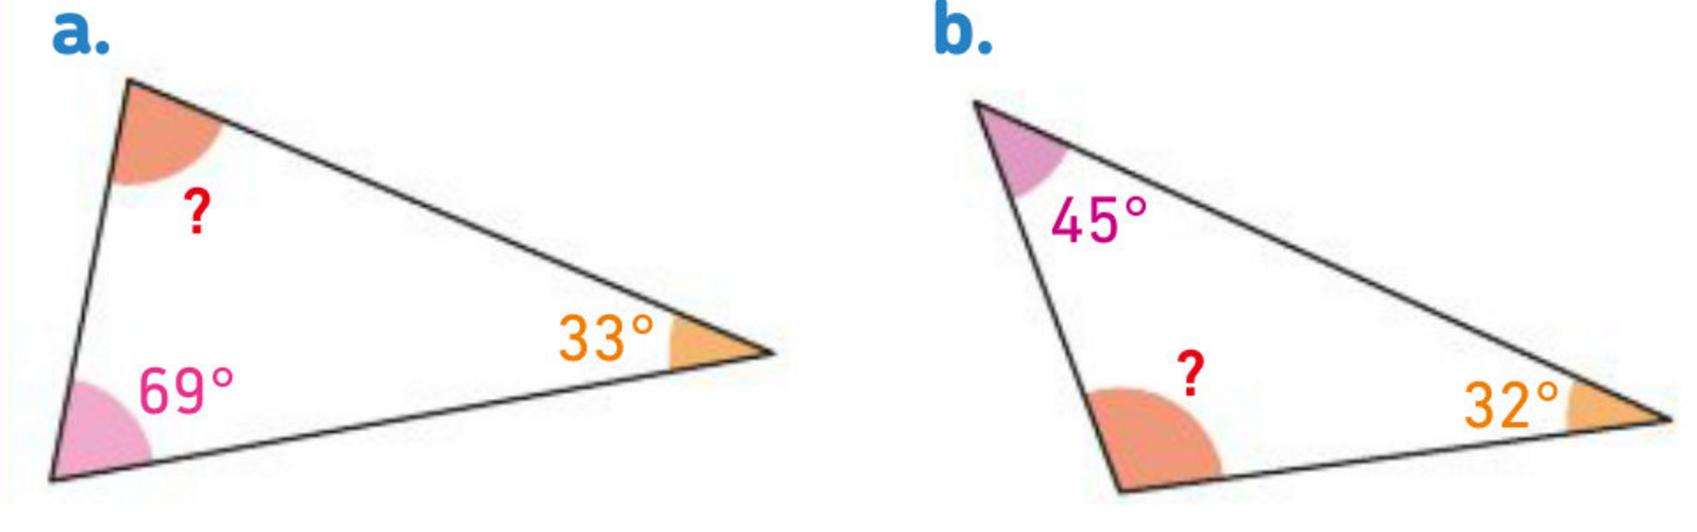
\includegraphics[scale=0.25]{../img/exos/45}\pause
	\end{center}	
	
	
	\begin{columns}
		\begin{column}{0.5\textwidth}
			\begin{eqnarray*}
				180 - (69 + 33) &=& 180 - 102 \\
				180 - (69 + 33) &=& 78\\
			\end{eqnarray*}
			
			L'angle mesure 78\degree.\pause
		\end{column}
	
		\begin{column}{0.5\textwidth}
			\begin{eqnarray*}
			180 - (45 + 32) &=& 180 - 77 \\
			180 - (45 + 32) &=& 103\\
			\end{eqnarray*}
		
			L'angle mesure 103\degree.
		\end{column}

	\end{columns}
\end{frame}

\begin{frame}
	\frametitle{Exercice 46 page 192}
	
	\begin{center}
		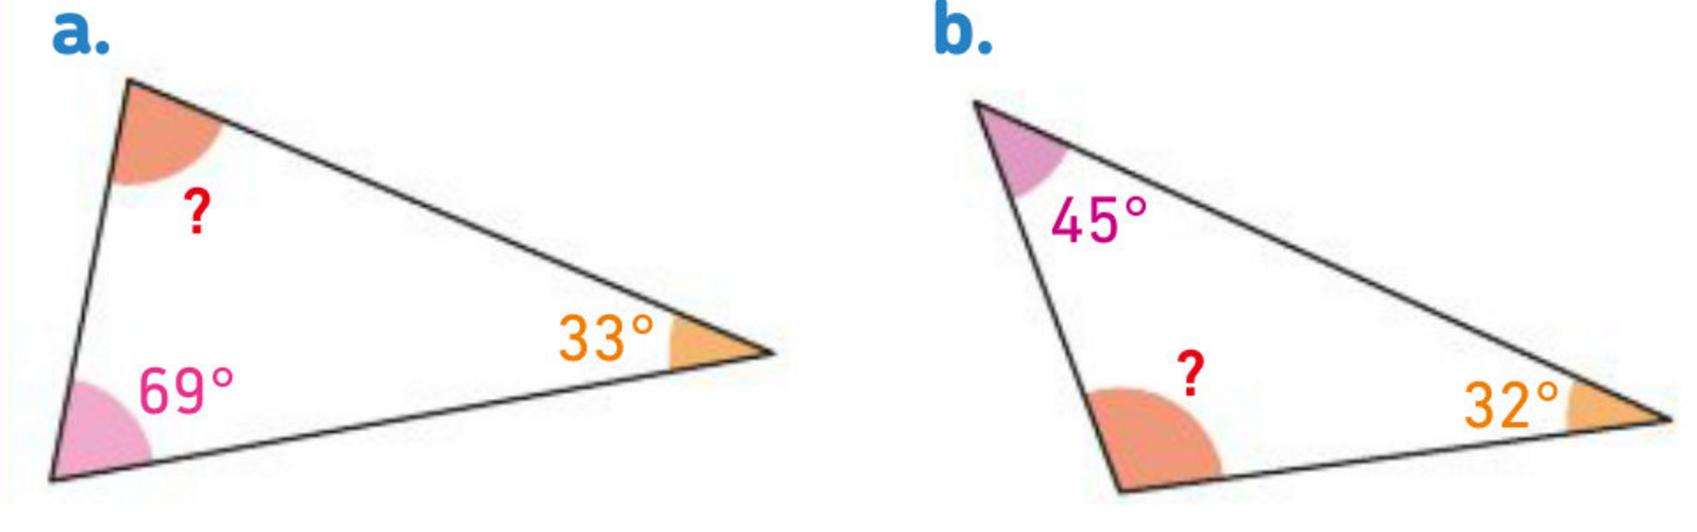
\includegraphics[scale=0.25]{../img/exos/45}\pause
	\end{center}	
	
	
	\begin{columns}
		\begin{column}{0.5\textwidth}
			\begin{eqnarray*}
				180 - (20 + 33) &=& 180 - 53 \\
				180 - (20 + 33) &=& 127\\
			\end{eqnarray*}
			
			L'angle mesure 127\degree.\pause
		\end{column}
		
		\begin{column}{0.5\textwidth}
			\begin{eqnarray*}
				180 - (25 + 114) &=& 180 - 139 \\
				180 - (45 + 32) &=& 41\\
			\end{eqnarray*}
			
			L'angle mesure 41\degree.
		\end{column}
		
	\end{columns}
\end{frame}


\begin{frame}
	%\frametitle{Exercice 46 page 192}
	
	\begin{block}{Exercice 48 page 192}
		Dans le triangle $AZE$, $\widehat{A} + \widehat{Z} + \widehat{E} = 180\degree$. \pause %Donc :\pause
		
		\vspace*{-0.5cm}
		\begin{eqnarray*}
			\widehat{E} &=& 180 - (57 + 31)\\ \pause
			%\widehat{E} &=& 180 - 88\\
			\widehat{E} &=& 92\\
		\end{eqnarray*}
		\vspace*{-0.75cm}
		
		L'angle $\widehat{E}$ mesure 92\degree.\pause
	\end{block}
	
	\begin{block}{Exercice 49 page 192}
		Dans le triangle $THG$, $\widehat{T} + \widehat{H} + \widehat{G} = 180\degree$.\pause %Donc :
		
		\vspace*{-0.5cm}
		\begin{eqnarray*}
		\widehat{G} &=& 180 - (103 + 29)\\
		%\widehat{G} &=& 180 - 132\\
		\widehat{G} &=& 48\\
		\end{eqnarray*}
		\vspace*{-0.75cm}
		
		L'angle $\widehat{G}$ mesure 48\degree.\pause
	\end{block}
	
	
	
\end{frame}

\begin{frame}
	%\frametitle{Exercice 46 page 192}
	
	\begin{block}{Exercice 51 page 192}
		
		La somme des mesures des angles d'un triangle vaut 180\degree. \pause  
		Le triangle est rectangle, un de ses angles mesure 90\degree et un autre 27\degree. \pause
		
		
		\begin{equation*}
			180 - (90 + 27) = 63
		\end{equation*}
%		\vspace*{-0.5cm}
%		\begin{eqnarray*}
%			\widehat{E} &=& \\ \pause
%			%\widehat{E} &=& 180 - 113\\
%			\widehat{E} &=& 63\\
%		\end{eqnarray*}
%		\vspace*{-0.75cm}
%		
		Les angles de ce triangle mesurent 90\degree, 27\degree et 63\degree. \pause
	\end{block}
	
	\begin{block}{Exercice 52 page 192}
		Le triangle $ABC$ est isocèle et rectangle en A, \pause l'angle $\widehat{A}$ mesure 90\degree et les deux autres sont égaux.
		Dans le triangle $ABC$, $\widehat{A} + \widehat{B} + \widehat{C} = 180\degree$.\pause %Donc :
		
		\vspace*{-0.5cm}
		\begin{eqnarray*}
			(180 - 90) \div 2 &=& 90 \div 2\\
			%\widehat{G} &=& 180 - 132\\
			(180 - 90) \div 2 &=& 45\\
		\end{eqnarray*}
		\vspace*{-0.75cm}
		
		Les angles $\widehat{A}$, $\widehat{B}$ et $\widehat{C}$ mesurent respectivement 90\degree, 45\degree et 45\degree.%\pause
	\end{block}
	
	
	
\end{frame}


\begin{frame}
	\frametitle{Exercice 54 page 193}
	

		Dans le triangle $ABD$, $\widehat{A} + \widehat{B} + \widehat{D} = 180\degree$.
		
		\vspace*{-0.5cm}
		\begin{eqnarray*}
			\widehat{D} &=& 180 - (67 + 56)\\ 
			%\widehat{E} &=& 180 - 88\\
			\widehat{D} &=& 57\\
		\end{eqnarray*}
		\vspace*{-0.75cm}
		
		L'angle $\widehat{ADB}$ mesure 57\degree. \pause
		
		Les points $B$, $D$ et $C$ sont alignés, l'angle $\widehat{BDC}$ mesure 180\degree. \pause Donc l'angle $\widehat{ADC}$ mesure 123\degree ($180 - 57$).\pause

		Dans le triangle $ADC$, $\widehat{A} + \widehat{D} + \widehat{C} = 180\degree$.
		
		\vspace*{-0.5cm}
		\begin{eqnarray*}
			\widehat{A} &=& 180 - (123 + 22)\\ 
			%\widehat{E} &=& 180 - 88\\
			\widehat{D} &=& 45\\
		\end{eqnarray*}
		\vspace*{-0.75cm}
		
		L'angle $\widehat{DAC}$ mesure 45\degree.
	
\end{frame}


\begin{frame}
	\frametitle{Exercice 55 page 193}
	
	
	\begin{enumerate}
		\item Dans un triangle isocèle, les angles à la base sont égaux.\pause
		
		
		\item \begin{enumerate}
			\item Le triangle $ABC$ est isocèle en A, les angles $\widehat{B}$ et $\widehat{C}$ sont égaux. Donc L'angle $\widehat{B}$ mesure 61\degree.\pause
			
			Dans le triangle $ABC$, $\widehat{A} + \widehat{B} + \widehat{C} = 180\degree$. Donc l'angle $\widehat{A}$ mesure 58\degree $(180 - 61 \times 2)$. \pause
			
			
			\item Le triangle $DEF$ est isocèle en E, les angles $\widehat{D}$ et $\widehat{F}$ sont égaux. \pause 
			La somme des mesures des angles d'un triangle vaut 180\degree. 
			Donc les angles $\widehat{E}$ et $\widehat{F}$ mesurent chacun 66\degree $((180 - 48) \div 2).$
		\end{enumerate}
	\end{enumerate}
\end{frame}
\end{document}